\documentclass[12pt,letterpaper]{exam}
\usepackage[lmargin=1in,rmargin=1in,tmargin=1in,bmargin=1in]{geometry}
\usepackage{../style/exams}

% -------------------
% Course & Exam Information
% -------------------
\newcommand{\course}{MATH 142: Final Exam}
\newcommand{\term}{Spring ---\textsubscript{\textsubscript{1}} 2026}
\newcommand{\examdate}{04/30/2026}
\newcommand{\timelimit}{150 Minutes}

\setbool{hideans}{false} % Student: True; Instructor: False

\newcommand{\boxseven}[4]{%
	\draw[thick] (0,0) -- (4,0) -- (4,4) -- (0,4) -- (0,0);
	\draw[thick] (0,2) -- (4,2);
	\draw[thick] (2,0) -- (2,4);
	% '7'
	\draw[line width=0.03cm] (1.7,2.2) -- (2.3,2.2) -- (1.7,1.6);
	% Entries
	\node at (1,3) {$#1$};	% u
	\node at (3,1) {$#2$};	% dv
	\node at (1,1) {$#3$};	% du
	\node at (3,3) {$#4$};	% v
}


\usetikzlibrary{calc}
\usepackage{booktabs}
\tikzset{Arrow Style/.style={text=black, font=\boldmath}}
\newcommand{\tikzmark}[1]{%
    \tikz[overlay, remember picture, baseline] \node (#1) {};%
}
\newcommand*{\XShift}{0.5em}
\newcommand*{\YShift}{0.5ex}
\NewDocumentCommand{\DrawArrow}{s O{} m m m}{%
    \begin{tikzpicture}[overlay,remember picture]
        \draw[->, thick, Arrow Style, #2] 
                ($(#3.west)+(\XShift,\YShift)$) -- 
                ($(#4.east)+(-\XShift,\YShift)$)
        node [midway,above] {#5};
    \end{tikzpicture}%
}

\usepackage{cancel}

% -------------------
% Content
% -------------------
\begin{document}

\examtitle
\instructions{Write your name on the appropriate line on the exam cover sheet. This exam contains \numpages\ pages (including this cover page) and \numquestions\ questions. Check that you have every page of the exam. Answer the questions in the spaces provided on the question sheets. Be sure to answer every part of each question and show all your work. If you run out of room for an answer, continue on the back of the page --- being sure to indicate the problem number.
} 
\scores
\bottomline
\newpage


% -------------------
% Questions
% -------------------
\begin{questions}

% --------------- Exam 1 --------------- %

% Question 1
\newpage
\question Showing all your work, complete the following:

\begin{parts}
% (a)
\part[5] Evaluate $\ds\int \cos^3 \theta \;d\theta$ \par\vspace{1.8cm}
\psol{\itshape Recall that $\sin^2 \theta + \cos^2 \theta= 1$, so $\cos^2 \theta= 1 - \sin^2 \theta$. We then have\dots}
	\[
	\psol{\int \cos^3 \theta \;d\theta= \int \cos^2 \theta \cdot \cos \theta \;d\theta= \int (1 - \sin^2 \theta) \cos \theta \;d\theta}
	\]
\psol{\itshape Now let $u= \sin \theta$, so that $du= \cos \theta \;d\theta$. But then\dots}
	\[
	\psol{\int \cos^3 \theta \;d\theta= \int (1 - \sin^2 \theta) \cos \theta \;d\theta= \int (1 - u^2) \;du= u - \dfrac{u^3}{3} + C= \sin \theta - \dfrac{\sin^3 \theta}{3} + C}
	\]
\psol{\itshape Therefore,}
	\[
	\psol{\boxed{\int \cos^3 \theta \;d\theta= \sin \theta - \dfrac{\sin^3 \theta}{3} + C}}
	\] \par\vspace{1.8cm}

% (b)
\part[5] Set-up but \textit{do not} evaluate an integral which computes the arclength of $y= \frac{2}{7} \, x^{7/2}$ on $[0, 1]$. \par\vspace{1cm}
\psol{\itshape The arclength of a differentiable function $f(x)$ on $[a, b]$ is $\ds L= \int_a^b \sqrt{1 + \big( f'(x) \big)^2} \;dx$. We have\dots}
	\[
	\begin{aligned}
	\psol{f(x)}&\psol{= \tfrac{2}{7}\, x^{7/2}} \\
	\psol{f'(x)}&\psol{= x^{5/2}} \\
	\psol{\big(f'(x) \big)^2}&\psol{= (x^{5/2})^2= x^5} \\
	\end{aligned}
	\]
\psol{\itshape We also have $[a, b]= [0, 1]$. Therefore, the arclength is given by\dots}
	\[
	\psol{\boxed{L= \int_0^1 \sqrt{1 + x^5} \;dx}}
	\] \vfill
\psol{\itshape\tiny Note. $\ds L= \int_0^1 \sqrt{1 + x^5} \;dx= {}_2F_1(-\tfrac{1}{2}, \tfrac{1}{5}, \tfrac{6}{5}, -1) \approx 1.07467$, where ${}_2F_1$ is the hypergeometric function.}
\end{parts}



% Question 2
\newpage
\question[10] Evaluate the integral below.
	\[
	\int \dfrac{1}{(\sqrt{16 - x^2})^3} \;dx
	\] 

\vsol{\itshape Because of the ``Pythagorean Theorem-like'' term $16 - x^2$, we use Trig. Substitution. From the Pythagorean Theorem, we know that $a^2 + b^2= c^2$. But then $b^2= c^2 - a^2$. Aligning corresponding terms, we want $c^2 - a^2= 16 - x^2$. So, we take $a^2= x^2$, i.e. $a= x$, and $c^2= 16$, i.e. $c= 4$. But then $b^2= c^2 - a^2= 16 - x^2$, so $b= \sqrt{16 - x^2}$. There are two possible right triangles corresponding to these sides we could draw:
	\[
	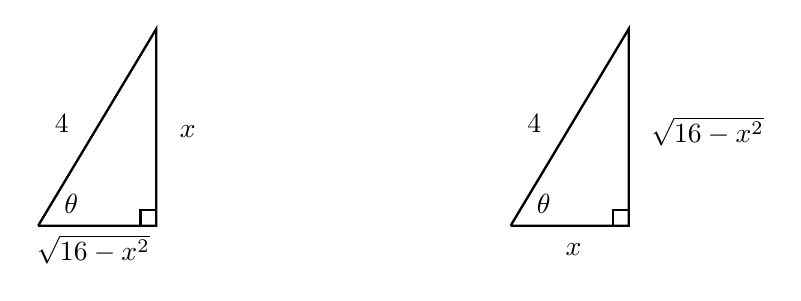
\begin{tikzpicture}
	\draw[line width=0.03cm] (0,0) -- (1.5,0) -- (1.5,2.5) -- (0,0);
	\draw[line width=0.03cm] (1.3,0) -- (1.3,0.2) -- (1.5,0.2);
	\node at (0.7,-0.3) {$\sqrt{16 - x^2}$};
	\node at (1.9,1.2) {$x$};
	\node at (0.3,1.3) {$4$};
	\node at (0.42,0.28) {$\theta$};
	
	\tikzset{shift={(6,0)}};

	\draw[line width=0.03cm] (0,0) -- (1.5,0) -- (1.5,2.5) -- (0,0);
	\draw[line width=0.03cm] (1.3,0) -- (1.3,0.2) -- (1.5,0.2);
	\node at (0.8,-0.3) {$x$};
	\node at (2.5,1.2) {$\sqrt{16 - x^2}$};
	\node at (0.3,1.3) {$4$};
	\node at (0.42,0.28) {$\theta$};
	\end{tikzpicture}
	\]
Using the triangle on the left, we see that $\sin \theta= \frac{x}{4}$, i.e. $x= 4 \sin \theta$. But then $dx= 4 \cos \theta \;d\theta$. We can also see from the triangle that $\cos \theta= \frac{\sqrt{16 - x^2}}{4}$, so that $\sqrt{16 - x^2}= 4 \cos \theta$. But then $(\sqrt{16 - x^2})^3= (4 \cos \theta)^3= 4^3 \cos^3 \theta$. Therefore, we have\dots
	\[
	\int \dfrac{1}{(\sqrt{16 - x^2})^3} \;dx= \int \dfrac{1}{4^3 \cos^3\theta} \cdot 4 \cos \theta \;d\theta= \int \dfrac{1}{4^{\cancel{3}^2} \cos^{\cancel{3}^2}\theta} \cdot \cancel{4}\, \cancel{\cos \theta} \;d\theta= \dfrac{1}{16} \int \dfrac{1}{\cos^2 \theta} \;d\theta
	\]
Using the fact that $\cos \theta= \frac{1}{\sec \theta}$, we know $\sec \theta= \frac{1}{\cos \theta}$ and $\sec^2 \theta= \frac{1}{\cos^2 \theta}$. But then\dots
	\[
	\int \dfrac{1}{(\sqrt{16 - x^2})^3} \;dx= \dfrac{1}{16} \int \dfrac{1}{\cos^2 \theta} \;d\theta= \dfrac{1}{16} \int \sec^2 \theta \;d\theta= \dfrac{1}{16} \tan \theta + C
	\]
From the right triangle, we see that $\tan \theta= \frac{x}{\sqrt{16 - x^2}}$. Therefore, we have\dots
	\[
	\int \dfrac{1}{(\sqrt{16 - x^2})^3} \;dx= \dfrac{1}{16} \tan \theta + C= \dfrac{1}{16} \cdot \frac{x}{\sqrt{16 - x^2}} + C= \boxed{\frac{x}{16\sqrt{16 - x^2}} + C}
	\] \par\vspace{0.2cm}
Alternatively, using the triangle on the right, we see that $\cos \theta= \frac{x}{4}$, i.e. $x= 4 \cos \theta$. But then $dx= -4 \sin \theta \;d\theta$. We can also see from the triangle that $\sin \theta= \frac{\sqrt{16 - x^2}}{4}$, so that $\sqrt{16 - x^2}= 4\sin \theta$. But then $(\sqrt{16 - x^2})^3= (4 \sin \theta)^3= 4^3 \sin^3 \theta$. Therefore, we have\dots
	\[
	\int \dfrac{1}{(\sqrt{16 - x^2})^3} \;dx= \int \dfrac{1}{4^3 \sin^3\theta} \cdot -4 \sin \theta \;d\theta= \int \dfrac{1}{4^{\cancel{3}^2} \sin^{\cancel{3}^2}\theta} \cdot \cancel{-4}^{\,-1}\, \cancel{\sin \theta} \;d\theta= -\dfrac{1}{16} \int \dfrac{1}{\sin^2 \theta} \;d\theta
	\]
Using the fact that $\csc \theta= \frac{1}{\sin \theta}$, we know $\csc^2= \frac{1}{\sin^2 \theta}$. But then\dots
	\[
	\int \dfrac{1}{(\sqrt{16 - x^2})^3} \;dx= -\dfrac{1}{16} \int \dfrac{1}{\sin^2 \theta} \;d\theta= \dfrac{1}{16} \int -\csc^2 \theta \;d\theta= \dfrac{1}{16} \cot \theta + C
	\]
From the right triangle, we see that $\cot \theta= \frac{x}{\sqrt{16 - x^2}}$. Therefore, we have\dots
	\[
	\int \dfrac{1}{(\sqrt{16 - x^2})^3} \;dx= \dfrac{1}{16} \cot \theta + C= \dfrac{1}{16} \cdot \frac{x}{\sqrt{16 - x^2}} + C= \boxed{\frac{x}{16\sqrt{16 - x^2}} + C}
	\]
}



% Question 3
\newpage
\question[10] Compute the following integral:
	\[
	\int \dfrac{13x - 8}{(x - 2)(x + 1)} \;dx
	\] \par\vspace{0.3cm}

\vsol{\itshape We use partial fractions. The degree of the numerator is 1 and the degree of the denominator is 2, so no long division is necessary. Observe the denominator is already fully factored. So, we can apply partial fractions decomposition. We have\dots
	\[
	\dfrac{13x - 8}{(x - 2)(x + 1)}= \dfrac{A}{x - 2} + \dfrac{B}{x + 1}
	\]
Combining terms on the right, we have\dots
	\[
	\dfrac{A}{x - 2} + \dfrac{B}{x + 1}= \dfrac{A(x + 1) + B(x - 2)}{(x - 2)(x + 1)}= \dfrac{Ax + A + Bx - 2B}{(x - 2)(x + 1)}= \dfrac{(A + B)x + (A - 2B)}{(x - 2)(x + 1)}
	\]
Because this must be equal to $\dfrac{13x - 8}{(x - 2)(x + 1)}$ and the two have the same denominator, their numerators must be equal. Equating like-terms in the numerators, we obtain the system of equations\dots
	\[
	\begin{cases}
	x\colon \quad A + B= 13 \\
	1\colon \quad A - 2B= -8
	\end{cases}
	\]
Subtracting the second equation from the first (so the $A$'s cancel), we have $3B= 21$, but then $B= 7$. From the first equation, we would then have $13= A + B= A + 7$, so $A= 6$. Alternatively, we could use Heaviside's Method (the Cover-Up Method). We would have\dots
	\[
	\begin{aligned}
	A&= \dfrac{13x - 8}{\boxed{\cancel{(x - 2)}} (x + 1)} \bigg|_{x= 2}= \dfrac{13(2) - 8}{2 + 1}= \dfrac{26 - 8}{3}= \dfrac{18}{3}= 6 \\
	B&= \dfrac{13x - 8}{(x - 2) \boxed{\cancel{(x + 1)}}} \bigg|_{x= -1}= \dfrac{13(-1) - 8}{-1 - 2}= \dfrac{-13 - 8}{-3}= \dfrac{-21}{-3}= 7
	\end{aligned}
	\]
Therefore, we have\dots
	\[
	\begin{aligned}
	\int \dfrac{13x - 8}{(x - 2)(x + 1)} \;dx= \int \left( \dfrac{6}{x - 2} + \dfrac{7}{x + 1} \right) \;dx= 6 \ln|x - 2| + 7 \ln|x + 1| + K
	\end{aligned}
	\]
Therefore, we have\dots
	\[
	\boxed{\int \dfrac{13x - 8}{(x - 2)(x + 1)} \;dx= 6 \ln|x - 2| + 7 \ln|x + 1| + K}
	\]
}



% Question 4
\newpage
\question[10] Showing all your work, compute the integral below.
	\[
	\int_0^\pi x \sin(7x) \;dx
	\] \par\vspace{0.3cm}

\vsol{\itshape\footnotesize We use Integration-by-Parts. Using LIATE, we choose $u= x$ (`A' for algebraic) and $dv= \sin(7x)$, i.e.
	\[
	\begin{tikzpicture}
	\boxseven{x}{\sin(7x)}{1}{-\dfrac{\cos(7x)}{7}}
	\end{tikzpicture}
	\]
So, we have\dots
	\[
	\begin{aligned}
	\int_0^\pi x \sin(7x) \;dx&= -\dfrac{x \cos(7x)}{7} \bigg|_0^\pi - \int_0^\pi -\dfrac{\cos(7x)}{7} \;dx \\[0.1cm]
	&= \left( -\dfrac{\pi \cos(7\pi)}{7} - \dfrac{-0 \cos(0)}{7} \right) + \dfrac{1}{7} \int_0^\pi \cos(7x) \;dx \\[0.1cm]
	&= - \dfrac{\pi(-1)}{7} + \dfrac{1}{7} \cdot \dfrac{\sin(7x)}{7} \bigg|_0^\pi \\[0.1cm]
	&= \dfrac{\pi}{7} + \dfrac{1}{49} \left( \sin(7\pi) - \sin(0) \right) \\[0.1cm]
	&= \dfrac{\pi}{7} + \dfrac{1}{49} \left( 0 - 0 \right) \\[0.1cm]
	&= \boxed{\dfrac{\pi}{7}}
	\end{aligned}
	\]
Alternatively, we can evaluate this integral using tabular integration: 
	\[
	\begin{array}{r @{\hspace*{1.3cm}} c} \toprule
	u & dv \\ \cmidrule(lr){1-2}
	x \tikzmark{Left 1} & \tikzmark{Right 1} \sin(7x) \\[0.3cm]
	1 \tikzmark{Left 2} & \tikzmark{Right 2} -\dfrac{\cos(7x)}{7} \\[0.3cm]
	0 \tikzmark{Left 3} & \tikzmark{Right 3} -\dfrac{\sin(7x)}{49}

	\DrawArrow{Left 1}{Right 2}{+}
	\DrawArrow{Left 2}{Right 3}{--}
	\end{array}
	\]
So that\dots
	\[
	\begin{aligned}
	\int_0^\pi x \sin(7x) \;dx&= \left( -\dfrac{x \cos(7x)}{7} + \dfrac{\sin(7x)}{49} \right) \bigg|_0^\pi \\[0.1cm]
	&= \left( -\dfrac{\pi \cos(7\pi)}{7} + \dfrac{\sin(7\pi)}{49} \right) - \left( -\dfrac{0 \cos(0)}{7} + \dfrac{\sin(0)}{49} \right) \\[0.1cm]
	&= \left( -\dfrac{\pi (-1))}{7} + \dfrac{\sin(0)}{49} \right) - \left( 0 + 0 \right) \\[0.1cm]
	&= \boxed{\dfrac{\pi}{7}}
	\end{aligned}
	\]

}



% Question 5
\newpage
\question[10] Determine whether the following improper integral converges or diverges. Be sure to fully justify your response.
	\[
	\int_0^\infty \dfrac{dx}{(x + 4)^2}
	\] \par\vspace{0.5cm}

\vsol{\itshape We have\dots
	\[
	\int \dfrac{dx}{(x + 4)^2}= -\dfrac{1}{x + 4} + C
	\] \par\vspace{0.5cm}
Therefore, we have\dots
	\[
	\begin{aligned}
	\int_0^\infty \dfrac{dx}{(x + 4)^2} &:= \lim_{b \to \infty} \int_0^b \dfrac{dx}{(x + 4)^2} \\[0.2cm]
	&= \lim_{b \to \infty} -\dfrac{1}{x + 4} \bigg|_0^b \\[0.2cm]
	&= \lim_{b \to \infty} -\dfrac{1}{b + 4} - \left( -\dfrac{1}{0 + 4} \right) \\[0.2cm]
	&= 0 - \left( -\dfrac{1}{4} \right) \\[0.2cm]
	&= \dfrac{1}{4}
	\end{aligned}
	\] \par\vspace{0.1cm}
Therefore, the integral converges to $\frac{1}{4}$. \par\vspace{0.5cm}
	\[
	\boxed{\int_0^\infty \dfrac{dx}{(x + 4)^2}= \dfrac{1}{4}}
	\]
}



% --------------- Exam 2 --------------- %



% Question 6
\newpage
\question Determine whether the following series converge or diverge. Be sure to fully justify your response. 

\begin{parts}
% (a)
\part[5] $\ds\sum_{n=1}^\infty \dfrac{3n + 5}{7n - 4}$ \par\vspace{1.3cm}
\psol{\itshape Observe\dots}
	\[
	\psol{\lim_{n \to \infty} \dfrac{3n + 5}{7n - 4}= \dfrac{3}{7} \neq 0}
	\] \par\vspace{0.5cm}
\psol{\itshape Therefore, $\ds\sum_{n=1}^\infty \dfrac{3n + 5}{7n - 4}$ diverges by the Divergence Test.} \par\vspace{5cm}

% (b)
\part[5] $\ds\sum_{n=0}^\infty \left( \dfrac{1}{2^k} - \dfrac{1}{2^{k+1}} \right)$ \par\vspace{0.2cm}
\psol{\itshape Observe that\dots}
	\[
	\begin{aligned}
	\sum_{n=0}^\infty \left( \dfrac{1}{2^k} - \dfrac{1}{2^{k+1}} \right)&= \lim_{N \to \infty} \sum_{n=0}^N \left( \dfrac{1}{2^k} - \dfrac{1}{2^{k+1}} \right) \\
	&= \lim_{N \to \infty} \left[ \left( \dfrac{1}{2^0} - \cancel{\dfrac{1}{2^{1}}} \right) + \left( \cancel{\dfrac{1}{2^1}} - \cancel{\dfrac{1}{2^{2}}} \right) + \left( \cancel{\dfrac{1}{2^2}} - \cancel{\dfrac{1}{2^{3}}} \right) + \cdots + \left( \cancel{\dfrac{1}{2^N}} - \dfrac{1}{2^{N+1}} \right) \right] \\
	&= \lim_{N \to \infty} \left[ 1 - \cancel{\dfrac{1}{2^{N+1}}}^0 \right] \\
	&= 1
	\end{aligned}
	\] \par\vspace{0.1cm}
\begin{center} \psol{\itshape OR} \end{center} \par\vspace{0.1cm}
	\[
	\sum_{n=0}^\infty \left( \dfrac{1}{2^k} - \dfrac{1}{2^{k+1}} \right)= \sum_{n=0}^\infty \left( \dfrac{2}{2^{k+1}} - \dfrac{1}{2^{k+1}} \right)= \sum_{n=0}^\infty \left( \dfrac{2 - 1}{2^{k+1}}\right)= \sum_{n=0}^\infty \left( \dfrac{1}{2^{k+1}}\right)= \sum_{n=0}^\infty \dfrac{1}{2} \left( \dfrac{1}{2} \right)^k
	\]
\psol{\itshape This series is geometric with $|r|= \frac{1}{2} < 1$. Therefore, the series converges by the Geometric Series Test. In fact, the sum would be $\dfrac{\;\;\tfrac{1}{2}\;\;}{1 - \tfrac{1}{2}}= \dfrac{\;\;\tfrac{1}{2}\;\;}{\tfrac{1}{2}}= 1$.}
\end{parts}



% Question 7
\newpage
\question[10] Determine whether the following series converges or diverges. Be sure to fully justify your response.  If the series converges, find its sum.
	\[
	\sum_{n=2}^\infty 3 \left(-\dfrac{2}{5} \right)^n
	\] \par\vspace{0.3cm}

\vsol{\itshape The series is geometric because the series has the form $\ds\sum^\infty ar^n$ with $a= 3$ and $r= -\frac{2}{5}$. Because $|r|= \frac{2}{5} < 1$, the series converges by the Geometric Series Test. We know that if a geometric series converges, it converges to $\frac{\text{first term}}{1 - r}$. Therefore, we have\dots
	\[
	\dfrac{\text{first term}}{1 - r}= \dfrac{3 \left( -\tfrac{2}{5} \right)^2}{1 - \left(- \tfrac{2}{5} \right)}= \dfrac{3 \cdot \tfrac{4}{25}}{1 + \tfrac{2}{5}} \cdot \dfrac{25}{25}= \dfrac{3 \cdot 4}{25 + 2(5)}= \dfrac{12}{25 + 10}= \dfrac{12}{35} \approx 0.342857
	\] \par\vspace{0.3cm}
	\[
	\boxed{\sum_{n=2}^\infty 3 \left(-\dfrac{2}{5} \right)^n \text{ converges by G.S.T. to } \frac{12}{35}}
	\]
}



% Question 8
\newpage
\question[10] Being sure to fully support your reasoning, determine whether the series given below converges or diverges.
	\[
	\sum_{n=1}^\infty \dfrac{(-1)^{n-1}}{7+2n}
	\] \par\vspace{0.3cm}

\vsol{\itshape Observe that the series is an alternating series. We have\dots
	\begin{itemize}
	\item $\ds\lim_{n \to \infty} \dfrac{1}{7+2n}= 0$: This function is rational. The degree of the denominator is 1 while the degree of the numerator is 0. Therefore, the limit at $\pm \infty$ is $0$.
	\item $\left\{ \dfrac{1}{7+2n} \right\}$ is decreasing: We need to show that $\{ a_n \}$ is decreasing, i.e. $a_{n+1} < a_n$. It is clear that $9 + 2n > 7 + 2n$, so that $\frac{1}{9 + 2n} < \frac{1}{7 + 2n}$. But $\frac{1}{9 + 2n}= \frac{1}{7 + 2 + 2n}= \frac{1}{7 + 2(n + 1)}$. But then $a_{n+1}= \frac{1}{7 + 2(n + 1)}= \frac{1}{9 + 2n} < \frac{1}{7 + 2n}= a_n$, so the sequence is decreasing. Alternatively, $\frac{d}{dx} \left( \frac{1}{7+2x} \right)= -\frac{2}{(7 + 2x)^2} < 0$ for all $x$. So, the sequence is decreasing. 
	\end{itemize}
Therefore, the series $\ds\sum_{n=1}^\infty \dfrac{(-1)^{n-1}}{7+2n}$ converges by the Alternating Series Test.
	\[
	\boxed{\sum_{n=1}^\infty \dfrac{(-1)^{n-1}}{7+2n} \text{ converges by A.S.T.}}
	\]
}



% Question 9
\newpage
\question Determine whether the following series converge or diverge. Be sure to fully justify your response. 

\begin{parts}
% (a)
\part[5] $\ds\sum_{n=0}^\infty \dfrac{(-3)^n}{n!}$ \par\vspace{1.75cm}
\psol{\itshape Using the Ratio Test, we have\dots}
	\[
	\psol{\hspace{-2.85cm} \lim_{n \to \infty} \left| \dfrac{\;\;\dfrac{(-3)^{n+1}}{(n+1)!}\;\;}{\dfrac{(-3)^n}{n!}} \right|= \lim_{n \to \infty} \dfrac{3^{n+1}}{(n+1)!} \cdot \dfrac{n!}{3^n} = \lim_{n \to \infty} \dfrac{3^{n+1}}{3^n} \cdot \dfrac{n!}{(n+1)!} = \lim_{n \to \infty} \dfrac{3^n \cdot 3}{3^n} \cdot \dfrac{n!}{(n+1)n!}= \lim_{n \to \infty} \dfrac{3}{n + 1}= 0 < 1}
	\] \par\vspace{0.3cm}
\psol{\itshape Therefore, the series converges absolutely by the Ratio Test.} \par\vspace{3.6cm}

% (b)
\part[5] $\ds\sum_{n=1}^\infty \left( \dfrac{3n + 4}{2n} \right)^n$ \par\vspace{1.75cm}
\psol{\itshape Using the Root Test, we have\dots}
	\[
	\psol{\lim_{n \to \infty} \left| \left( \dfrac{3n + 4}{2n} \right)^n \right|^{1/n}= \lim_{n \to \infty} \dfrac{3n + 4}{2n}= \dfrac{3}{2} > 1}
	\] \par\vspace{0.3cm}
\psol{\itshape Therefore, the series diverges by the Root Test.}
\end{parts}



% Question 10
\newpage
\question[10] Determine whether the series below diverges, converges conditionally, or converges absolutely. Include all necessary justifications. [Hint: $n > \ln(n + 1)$ for $n \geq 1$.] 
	\[
	\sum_{n=1}^\infty \dfrac{(-1)^n}{\ln(n + 1)}
	\] \par\vspace{0.3cm}
	
\vsol{\itshape Observe that the given series is alternating. We can also observe\dots
	\begin{itemize}
	\item $\ds\lim_{n \to \infty} \dfrac{1}{\ln(n + 1)}= 0$: This is obvious as the numerator is fixed but $\ds\lim_{n \to \infty} \ln(n + 1)= \infty$. 
	\item $\left\{ \dfrac{1}{\ln(n + 1)} \right\}$ is decreasing: We need to show that $a_{n + 1} < a_n$. Observe that $n + 1 > n$. As $\ln x$ is an increasing function, observe $\ln(n + 1) > \ln(n)$. But then $a_{n+1}= \frac{1}{\ln(n+1)} < \frac{1}{\ln n}= a_n$. So, the sequence is decreasing. Alternatively, observe that $\frac{d}{dx} \left( \tfrac{1}{\ln(x + 1)} \right)= -\tfrac{1}{(x + 1) [\ln(x + 1)]^2} < 0$ for $x > -1$. This also shows the sequence is decreasing.
	\end{itemize}
Therefore, the given series converges by the Alternating Series Test. \par\vspace{0.3cm}

Now we consider the series $\ds\sum_{n=1}^\infty \dfrac{1}{\ln(n + 1)}$. We know that $n > \ln(n + 1)$ for $n \geq 1$. But then $\frac{1}{n} < \frac{1}{\ln(n + 1)}$ for $n \geq 1$. But then we know\dots
	\[
	\sum_{n=1}^\infty \frac{1}{n} < \sum_{n=1}^\infty \frac{1}{\ln(n + 1)}
	\]
Because the series $\ds\sum_{n=1}^\infty \frac{1}{n}$ diverges by the $p$-test with $p= 1$. Alternatively, this is the Harmonic series, which we know diverges. But then the series $\ds\sum_{n=1}^\infty \frac{1}{\ln(n + 1)}$ diverges by the Direct Comparison Test. \par\vspace{0.3cm}

Because $\ds\sum_{n=1}^\infty \dfrac{(-1)^n}{\ln(n + 1)}$ converges but the series $\ds\sum_{n=1}^\infty \frac{1}{\ln(n + 1)}$ diverges, the series $\ds\sum_{n=1}^\infty \dfrac{(-1)^n}{\ln(n + 1)}$ converges conditionally. \par\vspace{0.5cm}
	\[
	\boxed{\sum_{n=1}^\infty \dfrac{(-1)^n}{\ln(n + 1)} \text{ converges conditionally}}
	\]	
}



% --------------- Exam 3 --------------- %



% Question 11
\newpage
\question Determine the center, radius, and interval of convergence for the following power series: \par\vspace{0.2cm}

\begin{parts}
% (a)
\part[5] $\ds\sum_{n=0}^\infty n! \, (x + 5)^n$ \par\vspace{0.3cm}
\psol{\itshape Using the Ratio Test, we have\dots}
	\[
	\psol{\lim_{n \to \infty} \left| \dfrac{(n + 1)! (x + 5)^{n+1}}{n! (x + 5)^n} \right|= \lim_{n \to \infty} \left| \dfrac{(n + 1)n! (x + 5)^n (x + 5)}{n! (x + 5)^n} \right|= \lim_{n \to \infty} | (n + 1)(x + 5)|= \infty}
	\]
\psol{Unless, of course, $x= -5$ (the center) in which case the series converges (it is $0$). So, the center is $x= -5$, the radius of convergence is $R= 0$, and the ``interval'' of convergence is $\{ 5 \}$.} \par\vspace{0.3cm}
	\wsol{%
	\[
	\boxed{%
	\begin{gathered}
	\text{Center: } x= -5 \\
	\text{``Interval'' of Convergence: } \{ 5 \} \\
	\text{Radius of Convergence: } R= 0
	\end{gathered}}
	\]%
	}
\par\vspace{2.3cm}

% (b)
\part[5] $\ds\sum_{n=0}^\infty \dfrac{x^n}{e^{n^2}}$ \quad [Hint: Use the Root Test] \par\vspace{0.3cm}
\psol{\itshape The center is $x= 0$. Using the Root Test, we have\dots}
	\[
	\psol{\lim_{n \to \infty} \left| \dfrac{x^n}{e^{n^2}} \right|^{1/n}= \lim_{n \to \infty} \left| \dfrac{x}{e^n} \right|= 0}
	\]
\psol{\itshape Therefore, the series converges for all $x$. So, the interval of convergence is $(-\infty, \infty)$, which means the radius of convergence is $R= \infty$.} \par\vspace{0.3cm}
	\wsol{%
	\[
	\boxed{%
	\begin{gathered}
	\text{Center: } x= 0 \\
	\text{Interval of Convergence: } (-\infty, \infty) \\
	\text{Radius of Convergence: } R= \infty
	\end{gathered}}
	\]%
	}
\end{parts}



% Question 12
\newpage
\question[10] Find the center, radius, and interval of convergence for the following power series:
	\[
	\sum_{n=1}^\infty \dfrac{(-1)^n}{2^n \sqrt{n}} \,(x - 1)^n
	\] \par\vspace{0.3cm}

\vsol{\itshape Clearly, the center is $x= 1$. We find the interval of convergence. Using the Ratio Test, we have\dots
	\[
	\begin{aligned}
	\lim_{n \to \infty} \left| \dfrac{\;\;\dfrac{(-1)^{n+1}}{2^{n+1} \sqrt{n+1}} \,(x - 1)^{n+1}\;\;}{\dfrac{(-1)^n}{2^n \sqrt{n}} \,(x - 1)^n} \right|&= \lim_{n \to \infty} \left| \dfrac{(x - 1)^{n+1}}{2^{n+1} \sqrt{n + 1}} \cdot \dfrac{2^n \sqrt{n}}{(x - 1)^n} \right| \\
	&=  \left| \dfrac{(x - 1)^{n+1}}{(x - 1)^n} \cdot \dfrac{2^n}{2^{n+1}} \cdot \dfrac{\sqrt{n}}{\sqrt{n + 1}} \right| \\
	&= \left| (x - 1) \cdot \dfrac{1}{2} \cdot \sqrt{\dfrac{n}{n + 1}} \right| \\
	&= \left| \dfrac{x - 1}{2} \right|
	\end{aligned}
	\]
Alternatively, using the Root Test, we have\dots
	\[
	\hspace{-1cm} \lim_{n \to \infty} \left| \dfrac{(-1)^n}{2^n \sqrt{n}} \,(x - 1)^n \right|^{1/n}= \lim_{n \to \infty} \left| \dfrac{1}{2 n^{1/(2n)}} \, (x - 1) \right|= \lim_{n \to \infty} \left| \dfrac{1}{2 (n^{1/n})^2} \, (x - 1) \right|= \left| \dfrac{1}{2(1)^2} (x - 1) \right|= \left| \dfrac{x - 1}{2} \right|
	\]
In either case, we know the series will converge if $\left| \dfrac{x - 1}{2} \right| < 1$, i.e. $-1 < \dfrac{x - 1}{2} < 1$. But then $-2 < x - 1< 2$, so that $-1 < x< 3$. Thus, the radius of convergence is $R= \frac{3 - (-1)}{2}= \frac{3 + 1}{2}= \frac{4}{2}= 2$. We now need to test the endpoints. \par\vspace{0.3cm}

$\underline{x= -1}$: If $x= -1$, the series is $\ds\sum_{n=1}^\infty \dfrac{(-1)^n}{2^n \sqrt{n}} \,(-1 - 1)^n= \sum_{n=1}^\infty \dfrac{(-1)^n}{2^n \sqrt{n}} \,(-2)^n= \sum_{n=1}^\infty \dfrac{(-1)^n (-1)^n}{\sqrt{n}}= \sum_{n=1}^\infty \dfrac{1}{\sqrt{n}}$. This series diverges by the $p$-test with $p= \frac{1}{2}$. \par\vspace{0.3cm}

$\underline{x= 3}$: If $x= 3$, the series is $\ds\sum_{n=1}^\infty \dfrac{(-1)^n}{2^n \sqrt{n}} \,(3 - 1)^n= \sum_{n=1}^\infty \dfrac{(-1)^n}{2^n \sqrt{n}} \,2^n= \sum_{n=1}^\infty \dfrac{(-1)^n}{\sqrt{n}}$. This series is alternating. We see $\ds\lim_{n \to \infty} \frac{1}{\sqrt{n}}= 0$ and the sequence $\left\{ \tfrac{1}{\sqrt{n}} \right\}$ is decreasing. Therefore, this series converges by the Alternating Series Test. \par\vspace{0.3cm}
	\[
	\boxed{%
	\begin{gathered}
	\text{Center: } x= 1 \\
	\text{Interval of Convergence: } (-1, 3] \\
	\text{Radius of Convergence: } R= 2
	\end{gathered}}
	\]
}



% Question 13
\newpage
\question[10] Find the third-degree Taylor polynomial, $T_3(x)$, for $f(x)= \sqrt{x}$ centered at $x= 1$. \par\vspace{0.3cm}

\vsol{\itshape We know that the Taylor series for a function $f(x)$ centered at $x= c$ is\dots
	\[
	T(x)= \sum_{n=0}^\infty \dfrac{f^{(n)}(c)}{n!} \, (x - c)^n
	\]
The center here is $c= 1$. We also want the third-degree Taylor polynomial, i.e. the terms of the Taylor series up to $n= 3$. Therefore, we have\dots
	\[
	\begin{aligned}
	T_3(x)&= \sum_{n=0}^3 \dfrac{f^{(n)}(1)}{n!} \, (x - 1)^n \\
	&= \dfrac{f^{(0)}(1)}{0!} \, (x - 1)^0 + \dfrac{f^{(1)}(1)}{1!} \, (x - 1)^1 + \dfrac{f^{(2)}(1)}{2!} \, (x - 1)^2 + \dfrac{f^{(3)}(1)}{3!} \, (x - 1)^3 \\
	&= f(1) + f'(1) (x - 1) + \dfrac{f''(1)}{2} \, (x - 1)^2 + \dfrac{f'''(1)}{6} \,(x - 1)^3
	\end{aligned}
	\]
We need only find these derivative values. We have\dots
	\[
	\begin{aligned}
	f(x)&= \sqrt{x} \bigg|_{x=1}= \sqrt{1}= 1 \\[0.2cm]
	f'(x)&= \dfrac{1}{2 \sqrt{x}} \bigg|_{x=1}= \dfrac{1}{2 \sqrt{1}}= \dfrac{1}{2} \\[0.2cm]
	f''(x)&= -\dfrac{1}{4 x^{3/2}} \bigg|_{x=1}= -\dfrac{1}{4(1^{3/2})}= -\dfrac{1}{4} \\[0.2cm]
	f'''(x)&= \dfrac{3}{8 x^{5/2}} \bigg|_{x=1}= \dfrac{3}{8 (1^{5/2})}= \dfrac{3}{8}
	\end{aligned}
	\]
Therefore, we have\dots
	\[
	\begin{aligned}
	T_3(x)&= f(1) + f'(1) (x - 1) + \dfrac{f''(1)}{2} \, (x - 1)^2 + \dfrac{f'''(1)}{6} \,(x - 1)^3 \\
	&= 1 + \dfrac{1}{2}\, (x - 1) + \dfrac{-1/4}{2} \, (x - 1)^2 + \dfrac{3/8}{6} \, (x - 1)^3 \\
	&= 1 + \dfrac{1}{2}\, (x - 1) - \dfrac{1}{8} \, (x - 1)^2 + \dfrac{1}{16} \, (x - 1)^3
	\end{aligned}
	\]
Therefore, we have\dots
	\[
	\boxed{T_3(x)= 1 + \dfrac{1}{2}\, (x - 1) - \dfrac{1}{8} \, (x - 1)^2 + \dfrac{1}{16} \, (x - 1)^3}
	\]
}



% Question 14
\newpage
\question Use a known Maclaurin series to find a\dots \par\vspace{0.2cm}

\begin{parts}
% (a)
\part[5] \dots power series representation for $\ds \dfrac{1}{1 + x^2}$. \par\vspace{0.3cm}
\psol{\itshape We know the Maclaurin series for $\dfrac{1}{1 - x}$ is $\ds\sum_{n=0}^\infty x^n$. But then the Maclaurin series for $\dfrac{1}{1 + x^2}$ is\dots}
	\[
	\psol{\dfrac{1}{1 + x^2}= \dfrac{1}{1 - (-x^2)}= \sum_{n=0}^\infty (-x^2)^n= \boxed{\sum_{n=0}^\infty (-1)^n \, x^{2n}}}
	\] \par\vspace{4.7cm}

% (b)
\part[5] \dots series approximation to $\ds \int_0^1 \ln(1 + x^2) \;dx$. \par\vspace{0.3cm}
\psol{\itshape We know the Maclaurin series for $\ds \ln(1 + x)= \sum_{n=1}^\infty (-1)^{n+1}\, \dfrac{x^n}{n}$ for $x \in (-1, 1]$. Observe that $x \in [0, 1]$, so that $x^2 \in [0, 1]$. But then\dots}
	\[
	\psol{\ln(1 + x^2)= \sum_{n=1}^\infty (-1)^{n+1}\, \dfrac{(x^2)^n}{n}= \sum_{n=1}^\infty (-1)^{n+1}\, \dfrac{x^{2n}}{n}}
	\]
\psol{\itshape But then\dots}
	\[
	\begin{aligned}
	\psol{\int_0^1 \ln(1 + x^2) \;dx}&= \psol{\int_0^1 \sum_{n=1}^\infty (-1)^{n+1}\, \dfrac{x^{2n}}{n} \;dx} \\
	&\psol{= \sum_{n=1}^\infty \int_0^1  (-1)^{n+1}\, \dfrac{x^{2n}}{n} \;dx} \\
	&\psol{= \sum_{n=1}^\infty (-1)^{n+1}\, \dfrac{x^{2n+1}}{n(2n +1)} \bigg|_0^1}  \\
	&\psol{= \sum_{n=1}^\infty \left( (-1)^{n+1}\, \dfrac{1^{2n+1}}{n(2n +1)} - (-1)^{n+1}\, \dfrac{0^{2n+1}}{n(2n +1)} \right)} \\
	&\psol{= \boxed{\sum_{n=1}^\infty (-1)^{n+1}\, \dfrac{1}{n(2n + 1)}} = \dfrac{\ln(4) + \pi - 4}{2} \approx 0.263944}
	\end{aligned}
	\]
\end{parts}



% Question 15
\newpage
\question[10] Determine the sum of the following series: \par\vspace{0.2cm}

\begin{enumerate}[(a)]
% (a)
\item $12 - 6 + 3 - \dfrac{3}{2} + \dfrac{3}{4} - \dfrac{3}{8} + \cdots$ \par\vspace{0.5cm}
\psol{\itshape\small Observe that each term in the sum/difference is $-\frac{1}{2}$ times the previous. Therefore, this series is geometric with common ratio $r= -\frac{1}{2}$ and first term $12$. Because $|r|= \frac{1}{2} < 1$, the sum converges. We know the sum is then $\frac{\text{first term}}{1 - r}= \frac{12}{1 - \left(-\frac{1}{2}\right)}= \frac{12}{1 + \frac{1}{2}}= \frac{12}{\frac{3}{2}} \cdot \frac{2}{2}= \frac{24}{3}= \boxed{8}$. Alternatively, we know that $\ds \dfrac{1}{1 - x}= \sum_{n=0}^\infty x^n$ for $x \in (-1, 1)$. But then $\ds \dfrac{12}{1 - x}= \sum_{n=0}^\infty 12x^n$ for $x \in (-1, 1)$. Observe the given series is this series with $x= -\frac{1}{2} \in (-1, 1)$. But then\dots}
	\[
	\psol{\hspace{-3.2cm}\resizebox{1.2\textwidth}{!}{$\ds 12 - 6 + 3 - \dfrac{3}{2} + \dfrac{3}{4} - \dfrac{3}{8} + \cdots= \sum_{n=0}^\infty 12 \left(-\dfrac{1}{2} \right)^n= \sum_{n=0}^\infty 12x^n \bigg|_{x=-\frac{1}{2}}= \dfrac{12}{1 - x} \bigg|_{x=-\frac{1}{2}}= \frac{12}{1 - \left(-\frac{1}{2}\right)}= \frac{12}{1 + \frac{1}{2}}= \frac{12}{\frac{3}{2}} \cdot \frac{2}{2}= \frac{24}{3}= \boxed{8}$}}
	\] \par\vspace{0.7cm}

% (b)
\item $\ds\sum_{n=0}^\infty (-1)^n \,\dfrac{(0.3)^{2n+1}}{(2n+1)!}$ \par\vspace{0.2cm}
\psol{\itshape\small We know that $\ds \sin x= \sum_{n=0}^\infty (-1)^n\, \dfrac{x^{2n+1}}{(2n+1)!}$ for all $x \in (-\infty, \infty)$. We know $x= 0.3 \in (-\infty, \infty)$. But then\dots}
	\[
	\psol{\sum_{n=0}^\infty (-1)^n \,\dfrac{(0.3)^{2n+1}}{(2n+1)!}= \sum_{n=0}^\infty (-1)^n \,\dfrac{x^{2n+1}}{(2n+1)!} \bigg|_{x=0.3}= \sin(x) \bigg|_{x=0.3}= \boxed{\sin(0.3)} \approx 0.29552}
	\]
\psol{\itshape\small Note. We would anticipate the value of the series to be approximately $0.3$ because we know $\sin \theta \approx \theta$ when $\theta \approx 0$.} \par\vspace{0.5cm}

% (c)
\item $1 - \dfrac{1}{2} + \dfrac{1}{3} - \dfrac{1}{4} + \dfrac{1}{5} - \dfrac{1}{6} + \cdots$ \par\vspace{0.3cm}
\psol{\itshape\small We know that $\ds\ln(1 + x)= \sum_{n=1}^\infty (-1)^{n+1}\, \dfrac{x^n}{n}$ for $x \in (-1, 1]$. But $x= 1 \in (-1, 1]$, so that\dots}
	\[
	\begin{aligned}
	\psol{1 - \dfrac{1}{2} + \dfrac{1}{3} - \dfrac{1}{4} + \dfrac{1}{5} - \dfrac{1}{6} + \cdots}&\psol{= \sum_{n=1}^\infty (-1)^{n+1}\, \dfrac{1}{n}} \\
	&\psol{= \sum_{n=1}^\infty (-1)^{n+1}\, \dfrac{x^n}{n} \bigg|_{x=1}} \\
	&\psol{= \ln(1 + x) \bigg|_{x=1}} \\
	&\psol{= \ln(1 + 1)} \\
	&\psol{= \boxed{\ln(2)} \approx 0.693147}
	\end{aligned}
	\]
\end{enumerate}

\end{questions}
\end{document}